%!TEX TS-program = xelatex

% Created by Gerson Sunyé on 2016-10-18.
% Copyright (c) 2016 .
\documentclass[a4]{report}

\usepackage{polyglossia}
\setdefaultlanguage{french}
%\usepackage{hyperref}
\usepackage{alma}
\usepackage{longtable}
\usepackage{graphicx}
\graphicspath{ {fig/} }
\usepackage{grffile}
\usepackage{lastpage}
\hypersetup
{
  pdftitle   = {Title},
  pdfsubject = {Subject},
  pdfauthor  = {Gerson Sunyé}
}
\newcommand{\projet}{Gestion des services}

\pagestyle{fancy}
\fancyhf{}
 \lhead{Master Informatique Alma/Atal}
 \chead{\includegraphics*[width=7mm]{fig/logo_mini.jpg}}
 \rhead{Université de Nantes}
 \cfoot{\scriptsize{G. Sunyé}}
 \lfoot{\scriptsize\textsl{\today}}
 \rfoot{\scriptsize\textsl{Page \thepage / \pageref{LastPage}}}
 \renewcommand{\footrulewidth} {0.4pt}


\fancypagestyle{empty}{
 \fancyhf{}
 \fancyhead[R]{Team \#3243 Page \thepage  { }of \pageref{LastPage}}
 \lhead{Master Informatique Alma/Atal}
 \chead{\includegraphics*[width=7mm]{fig/logo_mini.jpg}}
 \rhead{Université de Nantes}
 \cfoot{\scriptsize{G. Sunyé}}
 \lfoot{\scriptsize\textsl{\today}}
 \rfoot{\scriptsize\textsl{Page \thepage / \pageref{LastPage}}}}


\title{Projet «\projet»}
\author{Gerson Sunyé\\
\texttt{gerson.sunye@univ-nantes.fr}}

\begin{document}

\maketitle
\stepcounter{page}

\begin{abstract}
L’objectif de ce projet  est de fournir un outil réparti capable de gérer les services de différents enseignants.
\end{abstract}


\tableofcontents


\chapter{Introduction}
\section{Objectifs}
L’objectif de ce projet est de concevoir et de mettre en oeuvre un logiciel réparti permettant la gestion des services de différents enseignants.
Cette application pourra être utilisée de manière indépendante dans les différents départements de l’université, par les enseignants et les chefs de département, pour réaliser le choix des services de chacun des enseignants.

Pour répondre à ce besoin, vous disposez d'un document d'analyse du domaine, présentant de manière relativement complète le domaine “Gestion des services” au sein du département Informatique, d'un document de spécification des exigences logicielles et d'un dictionnaire de données, qui constitue une liste non-exhaustive de l’ensemble des termes relatifs au domaine étudié.
Des informations complémentaires pourront être fournies dans le forum de discussions dédié au projet.



\section{Prérequis}

Pour réaliser ce projet, l'étudiant doit maîtriser les langages et outils suivants:
\begin{enumerate}
	\item UML, le langage de modélisation unifié.
	\item OCL, le langage d'expression de contraintes de UML.
	\item Le langage Java, ou éventuellement  un langage JVM, comme Kotlin ou Groovy.
	\item Un outil de test unitaire de type xUnit: JUnit ou TestNG.
	\item Un outil pour la gestion et l'automatisation de production des projets logiciels Java, comme Apache Maven ou Gradle.
\end{enumerate}


\section{Travail à rendre}
Le projet se compose de deux livrables:
\begin{enumerate}
	\item Un document PDF contenant la description de la conception.
	\item Une archive contenant le code source.
\end{enumerate}

La conception de l'application sera composée de trois parties:
\begin{enumerate}
	\item L'architecture.
	\item La conception préliminaire (spécification des composants);
	\item La conception détaillée.
\end{enumerate} 

Les chapitres qui décrivent la conception doivent être organisés en fonction de la solution proposée (de ses fonctionnalités).
Suivez le modèle proposé dans ce document.


\section{Critères d'évaluation}

L'évaluation sera faite exclusivement sur le respect des exigences logicielles décrites dans le Chapitre~\ref{chapter:exigences}.
Lisez attentivement toutes les exigences avant de commencer votre projet.

\section{Organisation}

Règles à respecter pendant la réalisation du projet:

\begin{enumerate}
	\item La réalisation du projet sera faite par des groupes d'au moins 2 et au plus 4 étudiants.
	Les projets qui ne respectent pas cette règles ne seront pas évalués.

	\item Chaque groupe déposera ses livrables sur le serveur Madoc: \url{http://madoc.univ-nantes.fr/}, \textbf{exclusivement}.
	Les projets envoyés par un autre moyen ne seront pas évalués.
	En cas de problèmes avec le dépôt d'un fichier, envoyez un message au responsable du module.
	
	\item Pour éviter tout problème de compatibilité, les rapports seront rendus en format PDF, \textbf{exclusivement}.
	
	\item Le code source et les tests seront rendus en une archive \texttt{tar.gz}, qui contiendra aussi un fichier \texttt{pom.xml} (Maven) ou \texttt{build.gradle} (Gradle) permettant la compilation du système et le lancement de la validation. Vous pouvez préciser s'il s'agit d'un projet Eclipse, IDEA ou un autre.
	
	\item Les fichiers Java compilés (*.class) ainsi que les éventuelles bibliothèques utilisées ne doivent pas être rendus avec le code source.
\end{enumerate}

\section{Préambule}

Les sources de ce document sont disponibles sur l'adresse suivante:

\url{https://github.com/sunye/tp-gestion-services}

Si vous avez des commentaires sur le document ou si vous souhaitez me communiquer des erreurs, merci de le faire directement sur Github.
Vous pouvez aussi modifier directement les sources du document et m'envoyer ensuite un \emph{pull request}.


%!TEX root = ./sujet-projet.tex

\chapter{Spécification des exigences logicielles}\label{chapter:exigences}
% Template proposé par "The Unified Process for EDUcation (UPEDU)"
% http://www.yoopeedoo.org/upedu/

%Selon le wikipedia \url{http://fr.wikipedia.org/wiki/Exigence_(ingénierie)}
%De bonnes exigences doivent être :
% * Nécessaires – Elles doivent porter sur des éléments nécessaires, c'est-à-dire des éléments importants du système que d'autres composants du système ne pourraient pas compenser.
% * Non ambiguës – Elles doivent être susceptibles de n'avoir qu'une seule interprétation.
% * Concises – Elles doivent être énoncées dans un langage qui soit précis, bref et agréable à lire, et qui de plus communique l'essence de ce qui est exigé.
% * Cohérentes – Elles ne doivent pas contredire d'autres exigences établies, ni être contredites par d'autres exigences. De plus, elle doit, d'un énoncé d'exigence au suivant, utiliser des termes et un langage qui signifie la même chose.
% * Complètes – Elles doivent être énoncées entièrement en un endroit et d'une façon qui ne force pas le lecteur à regarder un texte supplémentaire pour savoir ce que l'exigence signifie.
% * Accessibles – Elles doivent être réalistes quant à aux moyens mis en œuvre en termes d'argent disponible, avec les ressources disponibles, dans le temps disponible.
% * Vérifiables – Elles doivent permettre de déterminer si elles ont été atteintes ou non selon l'une de quatre méthodes possibles : inspection, analyse, démonstration, ou test.

\section{Introduction}

Ce document énumère les exigences du projet «\projet{}». Il suit la norme IEEE 830-1998.


\subsection{Objectif}
%Préciser les objectifs de ce chapitre. La SEL doit décrire le comportement externe de l’application ou du sous-système identifié. Elle décrit aussi les exigences non-fonctionnelles et les autres facteurs nécessaires à une description complète et compréhensible des exigences pour le logiciel.
Ce document a pour objectif de décrire les exigences fonctionnelles et non-fonctionnelles du projet «\projet».
La description du comportement utilisateur attendu du système fera référence à l'analyse du domaine, présentée dans le Chapitre\ref{chapter:analyse}

\subsection{Portée du document}
Ce document s’applique seulement au développement de composants «métier» du système. Il ne concerne pas l’interface utilisateur.

\subsection{Définitions, acronymes et abréviations}


\begin{tabular}{ll}
\toprule
Acronyme & Description \\
\midrule
CM 			& Cours magistral\\
IHM 		& Interface Homme-Machine\\
REST 		& Representational State Transfer\\
TD			& Travaux dirigés\\
TP			& Travaux pratiques\\
\bottomrule
\end{tabular}

\subsection{Références}

\subsection{Vue d’ensemble} 

\subsection{Organisation du chapitre}
%Cette section décrit le contenu du reste du chapitre  et explique comment le document est organisé.

\section{Description générale}
%Décrire les principaux facteurs qui affectent le produit et ses exigences. On n’y énonce pas des exigences spécifiques, mais on y fournit une toile de fond aux exigences qui sont définies en détail à la section 3 afin d’en faciliter la compréhension. Cela comprend les items suivants:

Deux rôles se confrontent lors de la gestion des services: le département et les enseignants.
Le département doit:
\begin{itemize}
	\item Publier la liste des enseignants gérés par le département et donc y réalisant leur service.
A chaque enseignant est associée le nombre d’heures qu’il doit réaliser.
C’est en fait une fourchette MIN..MAX. Ces nombres varient d’un enseignant à l’autre et sont exprimés dans une unité eqTD (heures équivalentes Travaux Dirigés).
Pour information, 1h de cours représente 1h30 de TD, alors que 1h30 de TP représente 1h de TD.
	\item Publier la liste des enseignements qui doivent être couverts, avec les informations suivantes (cf. exemple Table~\ref{table:enseignements}):
	\begin{itemize}
		\item Nom du module.
		\item Publics concernés (année d’étude, parcours).
		\item Volume horaire par étudiants (Cours, TD, TP).
		\item Nombre de groupes (Cours, TD, TP).
		\item Semestre dans l’année universitaire.
	\end{itemize}
	\item Affecter les enseignants et visualiser leur nombres d’heures réalisées dans leur service (en éqTD) 
\end{itemize}

\begin{table}
	\begin{center}
	\begin{tabular}{lcrrrrrr}
	\toprule
	\textbf{Cours} & \textbf{Semestre} & \multicolumn{2}{c}\textbf{{CM}} & \multicolumn{2}{c}{\textbf{TD}} & \multicolumn{2}{c}{\textbf{TP}} \\
				& & \textbf{HE} & \textbf{nb} & \textbf{HE} & \textbf{nb} & \textbf{HE} & \textbf{nb} \\
	\midrule
	S4I0100 & 1 & 18 & 1 & 15 & 3 & 18 & 5 \\
	S3I0200 & 1 & 18 & 1 & 15 & 3 & 18 & 6 \\
	S1I0100 & 2 & 16 & 1 & 20 & 1 & -  & - \\
	S5I0400 & 2 & 5  & 1 & 20 & 1 & 20 & 2 \\
	\bottomrule
	\end{tabular}
	\end{center}
	\caption{Exemple de cours disponibles dans le département}
	\label{table:enseignements}
\end{table}

Les enseignants doivent:
\begin{itemize}
	\item Prendre connaissance des enseignements disponibles sur le département.
	\item Énoncer des préférences quant aux cours qu’ils souhaitent couvrir. Pour ce faire, un enseignant constitue la liste des enseignements qu’il souhaite couvrir en les classant du plus souhaité (en position 1) au moins souhaité (dernière position). Cf. Table~\ref{table:demande} pour un exemple. 
Pour être acceptable, une demande doit correspondre à un volume horaire au moins égale à 1,5 fois le service que doit effectuer l’enseignant.
	\item Prendre connaissance des préférences énoncées par les autres enseignants pour essayer de résoudre les problèmes éventuels autant que faire se peut.
	\item Prendre connaissance des cours qui leur ont été affectés, les préparer, les assurer.
\end{itemize}

\begin{table}
	\begin{center}
	\begin{tabular}{cccccc}
		\toprule
		\textbf{Num} & \textbf{Nom Module} & \textbf{Catégorie} & \textbf{Volume Etudiant} & \textbf{Nb groupes demandés} & \textbf{éqTD} \\
		\midrule
		1 & S4I0200 & CM & 15 & 1 & 22,5 \\
		2 & S4I0100 & TD & 18 & 1 & 18 \\
		3 & S4I0100 & TP & 15 & 2 & 20 \\
		\bottomrule
	\end{tabular}
	\end{center}
	\caption{Exemple de demande de service}
	\label{table:demande}
\end{table}



% \subsection{Perspectives du produit}
% %<Describe the context and origin of the product being specified in this SRS. For example, state whether this product is a follow-on member of a product family, a replacement for certain existing systems, or a new, self-contained product. If the SRS defines a component of a larger system, relate the requirements of the larger system to the functionality of this software and identify interfaces between the two. A simple diagram that shows the major components of the overall system, subsystem interconnections, and external interfaces can be helpful.>
%
% \subsubsection{Interfaces système}
% Le système ne communiquera pas avec d’autres systèmes.
%
% \subsubsection{Interfaces utilisateurs}
%
%
% \subsubsection{Interfaces matérielles}
% Aucune interface matérielle n’est exigée.
%
% \subsubsection{Interfaces logicielles}
%
%
% \subsubsection{Interfaces de communication}
% Le système ne communiquera avec aucun autre système ou serveur.
%
% \subsubsection{Contraintes de mémoire}
% Le système doit pouvoir s’exécuter correctement sur un ordinateur personnel disposant d'au moins 4Go de mémoire vive.


	\subsection{Fonctions du produit}
%Décrire brièvement les fonctions principales du logiciel. Par exemple : 
%Les fonctions d’un système de gestion peuvent être la maintenance d’un compte client, accéder à l’état de compte du client et produire la facturation.
Le système doit permettre aux enseignants de émettre des souhaits de service et au directeur du département de valider ces souhaits.
Il n’est pas question de réaliser un outil permettant d’optimiser automatiquement les affectations d’enseignants. 
C’est un outil d’aide à la gestion qui doit être proposé aux départements et aux enseignants.

Fonctionnalités souhaitées pour le département:
\begin{itemize}
	\item Mémorisation des services des années passées.
	\item Constitution de la liste des enseignements à couvrir.
	\item Récupération des choix des enseignants.
	\item Affichage des services suivant différent modes (globalement, par modules, par enseignants, par formation, seulement les souhaits, seulement les affectations effectives, les deux, etc.).
	\item Affectation des enseignants sur les enseignements.
	\item Alertes concernant:
\begin{itemize}
	\item les enseignements non couverts
	\item les enseignements trop demandés
	\item les conflits entre les demandes
	\item les enseignants n’entrant pas dans le cadre de leur contrat de service statutaire.
\end{itemize}
	\item La possibilité d’effectuer des affectations et des modifications sans les rendre publiques.
	\item La possibilité de valider un état courant, c'est à dire de le rendre public.
\end{itemize}

Fonctionnalités souhaitées pour les enseignants:

\begin{itemize}
	\item Mémorisation du service de l’enseignant des années passées, éventuellement ses choix.
	\item Récupération des choix des autres enseignants (globalement ou à la demande).
	\item Afficher les services suivant différent modes (globalement, par modules, par enseignants, par formation, seulement les souhaits, seulement les affectations effectives, les deux, etc.).
	\item Repérage facile des enseignements non encore demandés.
	\item Alertes concernant:
	\begin{itemize}
		\item les conflits entre les demandes
		\item les enseignants dépassant le minimum ou le maximum correspondant à leur contrat de service par rapport aux affectations réalisées. 
	Plus particulièrement pour l’enseignant connecté.
	\end{itemize}
	\item Alarmes lorsque l’affectation effective des services ne respecte pas les choix de l’enseignant.
	\item Publication du choix.
\end{itemize}


Attention, un enseignant doit pouvoir changer sa liste de choix à n’importe quel moment.

	
	\subsection{Caractéristiques et classes d'utilisateurs}
%Décrire les caractéristiques générales des utilisateurs qui ont un impact sur les exigences du document. Cela inclut le niveau de scolarité, l’expérience et l’expertise technique.
%<Identify the various user classes that you anticipate will use this product. User classes may be differentiated based on frequency of use, subset of product functions used, technical expertise, security or privilege levels, educational level, or experience. Describe the pertinent characteristics of each user class. Certain requirements may pertain only to certain user classes. Distinguish the favored user classes from those who are less important to satisfy.>

Les utilisateurs du système seront des enseignants avec une certaine maîtrise de l'informatique.

	\subsection{Environnement opérationnel}
%<Describe the environment in which the software will operate, including the hardware platform, operating system and versions, and any other software components or applications with which it must peacefully coexist.>

Le système sera déployé sur les machines des enseignants du département d'informatique: des ordinateurs de bureau et portables, sous Windows, Linux, OSX et FreeBSD.
Il sera utilisé lorsque les ordinateurs sont connectés sur un réseau ou déconnectés en mode nomade. 


%\subsection{Contraintes de plateforme}
%  Les contraintes de plateforme sont des contraintes liées à l'aspect matériel (coût d'achat, licence\dots).
%  Dans notre cas, nous nous sommes abstraits de la plupart de ces contraintes en décidant d'utiliser une plateforme gratuite et polyvalente : J2EE.\\
%
%  Java 2 Platform, Enterprise Edition est un framework pour le langage de programmation Java de Sun, plus particulièrement destiné aux applications d'entreprise. Dans ce but, il contient un ensemble d'extension au framework standard (JDK) afin de faciliter la création d'applications réparties. Notre application devant partager des bases de données, cette facilité nous avantage grandement.
%
%  Nous utilisons donc le langage Java qui est :
%  \begin{itemize}
%  \item Gratuit ;
%  \item multi-plateformes.
%  \end{itemize}
%
%  Les contraintes de plateforme sont ainsi limitées (cet environnement JAVA est librement téléchargable sur Internet).\\
%
%  Nous utilisons aussi le système de mapping Hibernate associé au SGBD ``Hypersonic SQL'' (libre d'utilisation et gratuit) pour la gestion de la persitence. Disponible sous forme de jar JAVA, il possède donc les même caractéristiques que celles mentionnées auparavant.\\
%
% De plus, la communication entre les différentes applications (système distribué) est assurée par le système CORBA (Common object request broker architecture), qui est destiné à permettre l'intercommunication entre tout système (multi-plateformes). Spécifié par l'OMG (Object management group) ce système est également libre d'utilisation et ne nécessite pas de licence.\\
%
%  Tous ces éléments sont tous librement disponibles sur Internet. Nous limitons ainsi les coûts associés aux contraintes de plateforme.


	\subsection{Contraintes de conception et de mise en œuvre}
%<Describe any items or issues that will limit the options available to the developers. These might include: corporate or regulatory policies; hardware limitations (timing requirements, memory requirements); interfaces to other applications; specific technologies, tools, and databases to be used; parallel operations; language requirements; communications protocols; security considerations; design conventions or programming standards (for example, if the customer’s organization will be responsible for maintaining the delivered software).>

	\subsubsection{Langage de programmation}
\begin{requirement}[Java]
	L’application doit être mise en œuvre dans le langages de programmation Java (version $\ge$ 1.7).
\end{requirement}


\subsubsection{Langage de conception}
\begin{requirement}[UML]
	Les diagrammes utilisés comme support à la conception doivent respecter la norme UML (version > 2.4) et le langage d’expression de contraintes OCL (version > 2.4).
\end{requirement}

\subsubsection{Conception}
La conception sera utilisée pour spécifier la mise en œuvre de la solution.

\begin{requirement}[{Conception claire}]
	La conception doit être claire et précise.
	Les diagrammes de conception doivent être systématiquement accompagnées d'une description textuelle.
\end{requirement}

\begin{requirement}[{Conception pour la testabilité}]
	La conception doit prioriser la testabilité: le code doit être facilement testable. 
\end{requirement}

\begin{requirement}[{Cohérence entre diagrammes}]
Les diagrammes de conception doivent être cohérents entre eux.
\end{requirement}

%La conception comprendra un diagramme de classes, des diagrammes d'objet et pour les opérations complexes, des diagrammes de séquence et d'activités. 

\subsubsection{Mise en œuvre}
\begin{requirement}[{Cohérence entre la conception et le code}]
La mise en œuvre doit être cohérente avec la conception.	
\end{requirement}

\begin{requirement}[{Lisibilité du code}]
Le code source doit être simple à comprendre et à évaluer: il doit être possible de les compiler et d'exécuter les tests unitaires à partir de la ligne de commandes.	
\end{requirement}



\subsubsection{Outils de construction}
\begin{requirement}[{Construction automatique}]
	L’utilisation d’outil de construction automatique est obligatoire: Maven ou Gradle.
\end{requirement}

\subsubsection{Outils de développement}
\begin{requirement}[{IDE}]
	L’utilisation d’un environnement de développement (IDE) compatible avec Maven ou Gradle, comme IntelliJ IDEA ou NetBeans, est fortement recommandée. 
\end{requirement}

\subsubsection{Bibliothèques et composants logiciels}
Les tests unitaires doivent utiliser JUnit (version > 4.10) ou son équivalent pour les autres langages de programmation.


	\subsection{Documentation utilisateur}
%<List the user documentation components (such as user manuals, on-line help, and tutorials) that will be delivered along with the software. Identify any known user documentation delivery formats or standards.>

	\subsection{Hypothèses et dépendances}
%Décrire tout élément de faisabilité technique, disponibilité de sous-système ou de composant ou toute autre hypothèse liée au projet de laquelle dépend la viabilité du logiciel.
	
%<List any assumed factors (as opposed to known facts) that could affect the requirements stated in the SRS. These could include third-party or commercial components that you plan to use, issues around the development or operating environment, or constraints. The project could be affected if these assumptions are incorrect, are not shared, or change. Also identify any dependencies the project has on external factors, such as software components that you intend to reuse from another project, unless they are already documented elsewhere (for example, in the vision and scope document or the project plan).>

\subsection{Exigences reportées}
%Énumérer les exigences qui peuvent être réalisées dans des versions futures du système.
% Les versions futures du système comprendront l’utilisation d’un mécanisme de persistance de données ainsi que différentes interfaces utilisateur: web, IHM classique, etc.
% Elles permettront aussi l’accès distant à travers une interface REST.

\begin{requirement}[{Import/export CSV}]
	Le système permettra l'importation et l'exportation de données au format CSV.
\end{requirement}

\begin{requirement}[{Interface graphique}]
	Le système sera accessible grâce à une interface graphique simple et ergonomique. 
\end{requirement}

\begin{requirement}[{Interface Web}]
	Le système sera accessible à travers une interface web.
\end{requirement}



\section{Exigences fonctionnelles}
%Décrire les exigences fonctionnelles du système qui peuvent être exprimées et langage naturel. Pour plusieurs applications, c’est la partie principale de la SEL et son organisation doit, par conséquent, être bien réfléchie. Elle est habituellement hiérarchisée par caractéristiques, mais elle peut l’être, par utilisateur ou par sous-système. Les exigences fonctionnelles peuvent inclure les caractéristiques, les capacités et la sécurité.

%Lorsque des outils de développement, tels des référentiels d’exigences ou des outils de modélisation sont utilisés, on peut référer à ces données en indiquant l’endroit et le nom de cet outil]


\subsection{\nameref{usecase:affecter}}
\begin{requirement}[Affectation]
	Confirmation, par le chef du département, d'un souhait d'un enseignant.
\end{requirement}

\subsection{\nameref{usecase:publier}}
\begin{requirement}[Publication des interventions]
	Le système doit permettre au chef du département de publier des interventions, des souhaits et des conflits.
\end{requirement}

\subsection{\nameref{usecase:analyse}}
\begin{requirement}[Analyse]
	Le système doit aider le chef du département à analyser les souhaits pour détecter des enseignants en sous-services et des modules non pourvus. 
\end{requirement}

\subsection{\nameref{usecase:souhait}}
\begin{requirement}[Expression de souhaits]
	Le système doit permettre aux enseignants d'émettre ses souhaits d'enseignement.
\end{requirement}

\subsection{\nameref{usecase:publier}}
\begin{requirement}[Publication de souhaits]
	Le système doit permettre aux enseignants de publier leurs souhaits.
\end{requirement}

\subsection{\nameref{usecase:consulter}}
\begin{requirement}[Consultation des enseignements]
	Le système doit permettre aux enseignants de consulter les enseignements.
\end{requirement}

\section{Exigences non-fonctionnelles}\label{section:non-fonctionnelles}
	\subsection{Interface utilisateur}
%<Describe the logical characteristics of each interface between the software product and the users. This may include sample screen images, any GUI standards or product family style guides that are to be followed, screen layout constraints, standard buttons and functions (e.g., help) that will appear on every screen, keyboard shortcuts, error message display standards, and so on. Define the software components for which a user interface is needed. Details of the user interface design should be documented in a separate user interface specification.>
Le système se résume à des composants sans interface utilisateur. 
Le bon fonctionnement des composants sera validé par des tests unitaires.

	\subsection{Interface matérielle}
%<Describe the logical and physical characteristics of each interface between the software product and the hardware components of the system. This may include the supported device types, the nature of the data and control interactions between the software and the hardware, and communication protocols to be used.>
Non applicable.

	\subsection{Interface logicielle}
%<Describe the connections between this product and other specific software components (name and version), including databases, operating systems, tools, libraries, and integrated commercial components. Identify the data items or messages coming into the system and going out and describe the purpose of each. Describe the services needed and the nature of communications. Refer to documents that describe detailed application programming interface protocols. Identify data that will be shared across software components. If the data sharing mechanism must be implemented in a specific way (for example, use of a global data area in a multitasking operating system), specify this as an implementation constraint.>

\begin{requirement}[Clarté des interfaces des composants]
	Le système doit être divisé en composants disposant d’interfaces logicielles claires et simples.
\end{requirement}

	\subsection{Interfaces ou protocoles de communication}
	
%<Describe the requirements associated with any communications functions required by this product, including e-mail, web browser, network server communications protocols, electronic forms, and so on. Define any pertinent message formatting. Identify any communication standards that will be used, such as FTP or HTTP. Specify any communication security or encryption issues, data transfer rates, and synchronization mechanisms.>
\begin{requirement}[Protocoles ouverts]
	La communication entre les différents composants du système doit utiliser des protocoles ouverts et disponibles sur différentes plateformes.
\end{requirement}

	\subsection{Contraintes de mémoire}
Non applicable.

\subsection{Hypothèses et dépendances}

%\section{Autres exigences non-fonctionnelles}

\subsection{Correction}
 La gestion des conflits étant problématique, il convient d'avoir une application fortement exacte, notamment au niveau de la communication entre les différents utilisateurs (d'autant plus qu'il s'agit d'une application distribuée). 
%Mais cette distribution implique que l'exactitude ne pourra pas, dans certains cas, être parfaite (un serveur, un réseau peuvent tomber\dots).

\begin{requirement}[Correction]
	La correction de toutes les opérations de tous les classes du système doit être vérifiée par des tests unitaires. 
	Plus particulièrement, les interfaces fournies par les composant doivent être testées de manière exhaustive.
\end{requirement}


 \subsection{Interopérabilité}
Il est aussi difficile de supposer que toutes les applications fonctionnent sur les mêmes systèmes ou sont programmées dans les mêmes langages.
Comme l'application doit interroger des bases distantes, elles-mêmes pouvant être gérées par un autre logiciel similaire, nous devons assurer une interopérabilité totale. 
 
\begin{requirement}[Interopérabilité]
	Le système doit être interopérable avec d'autres systèmes.
\end{requirement}
 

\subsection{Portabilité}
\begin{requirement}[Portabilité]
	L'application doit pouvoir s'appliquer à tous les systèmes d'exploitation, donc, le logiciel doit être complètement portable.
\end{requirement}



\subsection{Exigences de performance}
L'application ne nécessite pas de performances particulières (du fait de l'utilisation par un homme) mais nous devons tout de même assurer des temps de réponse raisonnables aux demandes de consultation des bases distantes.
	
	%
	% Décrire les caractéristiques de la performance du système. Référer les cas d’utilisation lorsque applicable.
	%
	% \begin{itemize}
	% \item	Temps de réponse par transaction (moyen, maximum)
	% \item	Débit (transactions par seconde)
	% \item	Capacité (nombre de client ou de transaction que le système doit supporter)
	% \item	Mode d’opération lors de dégradation (Mode d’opération acceptable lorsque la performance du système se détériore)
	% \item	Utilisation de ressources (mémoire, disque, communications, etc.
	% \end{itemize}
	%
	% \subsubsection{Nom de l’exigence de performance 1}
	% Description de l’exigence

\subsection{Maintenabilité}
	
%Décrire les exigences qui permettent d’assurer le support et la maintenabilité du système comme, par exemple, les normes de codage, le conventions d’identification, les bibliothèques de classe, l’accès à la maintenance, les services de maintenances, etc. 

\subsubsection{Conventions de code Java}

\begin{requirement}[Conventions de codage]
	Le code source Java doit respecter le style proposé par Google:\\
\url{https://google.github.io/styleguide/javaguide.html}
\end{requirement}


	% \subsubsection{Nom de l’exigence de maintenabilité 1}
	% Description de l’exigence

	\subsection{Exigences de sûreté}
%<Specify those requirements that are concerned with possible loss, damage, or harm that could result from the use of the product. Define any safeguards or actions that must be taken, as well as actions that must be prevented. Refer to any external policies or regulations that state safety issues that affect the product’s design or use. Define any safety certifications that must be satisfied.>

	\subsection{Exigences de sécurité}
	% Identifier les données qui doivent être protégées et le type de menace auquel elles sont exposées comme, par exemple, menaces physiques, types de personnes qui peuvent être la source de menace, les exigences d’accès au système, l’encryptage des données, la vérifiabilité qui est la détection des anomalies et des opérations frauduleuses.
	%
	% Énumérer la liste des objets qui doivent faire l’objet d’une protection physique ou logique

La sécurité influe beaucoup sur la performance d'exécution. Cette dernière n'étant pas prioritaire, nous pouvons demander une forte sécurité (bien que les données manipulées ne soient pas particulièrement sensibles).

\begin{requirement}[Identification]
	Le logiciel doit permettre d'identifier et authentifier les différentes applications des différentes personnes.
\end{requirement}

\subsection{Attributs de qualité logicielle}
	
%<Specify any additional quality characteristics for the product that will be important to either the customers or the developers. Some to consider are: adaptability, availability, correctness, flexibility, interoperability, maintainability, portability, reliability, reusability, robustness, testability, and usability. Write these to be specific, quantitative, and verifiable when possible. At the least, clarify the relative preferences for various attributes, such as ease of use over ease of learning.>

\section{Autres exigences}
%<Define any other requirements not covered elsewhere in the SRS. This might include database requirements, internationalization requirements, legal requirements, reuse objectives for the project, and so on. Add any new sections that are pertinent to the project.>

\subsection{Persistance}

\begin{requirement}[Persistance]
	Les données saisies par le département doivent être persistances. En particulier, les demandes non-publiées des enseignants.
\end{requirement}

% L’application d’utilisateur doit fonctionner même lorsque ce dernier est déconnecté en particulier pour communiquer ses choix aux différentes personnes les sollicitant.


\subsection{Système réparti}

\begin{requirement}[Informatique nomade]
	Un utilisateur doit pouvoir consulter et modifier l’état de sa déclaration de service avec son application où qu’il se trouve, même s'il n'est pas connecté à un réseau.
\end{requirement}

\begin{requirement}[Localisation des applications]
	Il n’est pas raisonnable de supposer que tous les composants soient hébergées sur la même machine.
	Il est donc nécessaire de les localiser.
\end{requirement}

\subsection{Outils de développement}

\begin{requirement}[Contrôle de version]
	Le développement du code source du logiciel doit utiliser un système de gestion de versions comme Git ou Subversion.
\end{requirement}

\begin{requirement}[UML Designer]
	Les diagrammes de conception doivent être réalisés sur Eclipse, avec UML Designer de Obeo.
\end{requirement}

\begin{requirement}[Spring]
	Le développement des composants doit se faire grâce au framework Spring.
\end{requirement}

\renewcommand{\listtheoremname}{Liste des exigences}

\listoftheorems[ignoreall,show={requirement}]

%\section{Conclusion}

%!TEX root = ./sujet-projet.tex

\chapter{Analyse du domaine}\label{chapter:analyse}
\section{Introduction}

Dans ce chapitre, nous présentons l'ensemble des cas d'utilisation que nous avons dégagés lors de l'analyse du domaine. Nous utiliserons pour cela le canevas proposé par Cockburn~\cite{Cockburn:2000} que nous compléterons par des instantanés ainsi que par des post-conditions exprimées en OCL (Object Constraint Language) et quelques scenarii. Cette partie constitue une étape clé de la phase de spécification des besoins. 

Nous présentons également le diagramme des classes métiers (i.e., le diagramme de classes au niveau analyse) que nous avons construit à partir de l'analyse réalisée jusqu'à présent. 
Ce diagramme fournit une vue statique et synthétique du domaine ``\projet'' de notre application. 
Cette dernière partie constitue également une étape clé de la phase de spécification des besoins.


\section{Définition des cas d'utilisation}
Dans cette section, nous spécifions  l'ensemble des cas d'utilisation relatifs au domaine ``\projet''. Le diagramme présenté dans la Figure~\ref{fig:usecases} résume l'ensemble des cas d'utilisation associés de notre système. Ceux-ci peuvent être effectués par deux acteurs différents:
 \begin{itemize}
 \item Le chef de département;
 \item l'enseignant.
 \end{itemize}

\begin{figure}[h!]
	\centering
		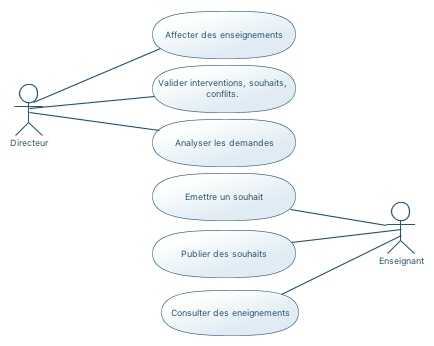
\includegraphics[scale=.7]{UC-Gestion Services.jpg}
	\caption{Cas d'utilisation du domaine "\projet".}
	 \label{fig:usecases}
\end{figure}

Dans les sections suivantes, nous fournissons une description plus détaillée de chacun des cas d'utilisation.

\subsection{UC---Affecter des enseignements}

\begin{usecase}{Affecter des enseignements}\label{usecase:affecter}
\begin{information}

 \item[Goal in the context:] Le chef de département réalise la confirmation d'un souhait d'un enseignant (validation) ou impose une intervention dans le département à un enseignant (affectation "forcée"). 
 L'enseignant devra se soumettre aux décisions du chef de département que ce soit pour une validation d'un souhait ou une affectation imposée.

\item[Scope:] Département

\item[{Level:}] Résumé (Summary)

 \item[{Precondition:}]
Le chef de département connait les souhaits (seulement ceux déjà publiés par l'enseignant), les possibles conflits et les affectations de l'enseignant concerné.

 \item[{Success End Condition:}]
L'enseignant est affecté à un ou plusieurs enseignements (souhait validé ou intervention imposée). 
Le volume horaire total effectué par l'enseignant a été recalculé.

 \item[{Failed End Condition:}]
 L'affectation n'a pas été réalisée (l'enseignement est déjà affecté à un autre enseignant : conflit).

\item[Primary actor:]
Chef de département.

 \item[Trigger:] Demande de réalisation d'une affectation faite par le chef de département.
\end{information}

\begin{scenario}
\item Le chef de département visualise l'ensemble des souhaits publiés par les enseignants.
\item Le chef de département sélectionne des souhaits, selon certains critères (l'enseignant, le module concerné, \dots).
%\item Le système renvoie les souhaits correspondants aux critères.  
\item Le chef de département choisit un vœu d'un enseignant afin de le valider.
\item Le chef de département valide le vœu, l'enseignement associé au vœu est affecté à l'enseignant concerné: c'est-à-dire que le vœu donne lieu à une intervention effective.
\item Le volume horaire des enseignants concernés est recalculé. 
\end{scenario}

 \begin{variation}
 \item [4] Le chef de département impose une intervention à un enseignant dans son département (affectation imposée).
 \item [4] Le chef de département valide une demande d'intervention extérieure ou une demande spéciale (remplacement, encadrement de stage, congés, \dots) de l'enseignant.
 % \item [4b1] Le système affecte l'intervention ou valide la demande spéciale de l'enseignant sans créer de conflits avec les autres enseignants.
 \end{variation}
\end{usecase}

\subsubsection{Spécification OCL}
\begin{ocl}
context UC::AffecterEnseignements(dep:Departement, voeux:Voeu[*])
post:
voeux->forAll(each:Voeux| let int = each.intervention in
	int.oclIsNew() and int.enseignant = each.enseignant and
	int.enseignement = each.enseignement)
	-- l`affectation d`un voeux crée une intervention dont l`enseignant et l`enseignement sont les mêmes que ceux du voeux.
 \end{ocl}

\begin{ocl}
context UC::AffecterDemandeExterieure(dep:Departement, d:DemandeExterieure)
post: let i = d.intervention in
	i.oclIsNew() and t.enseignement = d.enseignant and
	dep.interventions->includes(d.intervention)
-- l'affectaton d'une demande extérieure donne lieu à une intervention extérieure qui fait parti de 
-- la liste d'affectation de l'enseignant (celui qui a émis cette demande). 
-- Cette affectation est effectuée par le département.
\end{ocl}

\begin{ocl}
context UC::AffecterDemandeSpeciale(dep:Departement, ds:DemandeSpeciale)
post: let speciale = ds.intervention in
	speciale.oclIsNew() and speciale.enseignant = ds.enseignant
-- La DemandeSpeciale réalisée donne lieu à un CasSpecial qui fait parti de la liste d`affectation 
-- de l`enseignant (celui qui a émis cete DemandeSpeciale : de.emet). 
-- Cette réalisation est effectuée par le  département.
\end{ocl}

\begin{ocl}
context Departement::imposeInterventionDepartement(dep:Departement, ens:Enseignant, e:Enseignement)
post: Intervention.allInstances()->exists(i : Intervention |
	i.oclIsNew() and i.enseignement = e and i.enseignant = e)
-- L`enseignement est lié à une unique InterventionDepartement qui appartient à la liste des affectations 
-- de l'enseignant ens. C'est le département qui impose cette Intervention.
\end{ocl}


\subsubsection{Exemple d'affectation de voeux}
La Figure~\ref{fig:affectation} présente un exemple d'affectation des 3 voeux d'Alice et Bob.
L'affectation donne lieux à la création de trois instances d'intervention.

\begin{figure}[!htbp]
\begin{center}
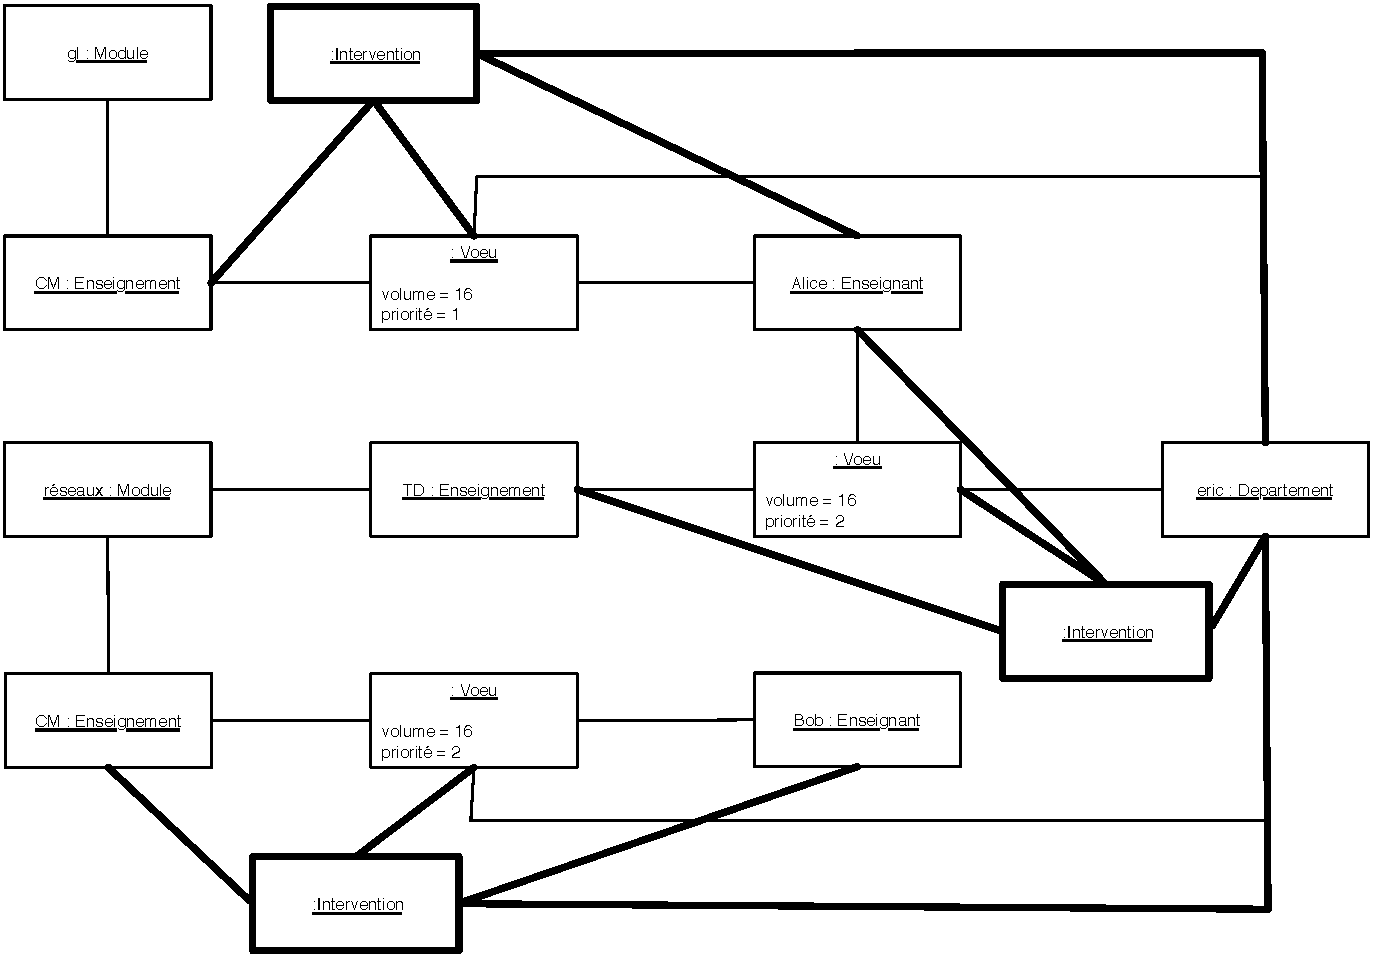
\includegraphics[scale=.6]{OD-affecter-voeux}
\caption{Diagramme d'objets: Affecter des vœux}\label{fig:affectation}
\end{center}
\end{figure}

\subsubsection{Exemple d'affectation à partir d'une demande extérieure}
La Figure~\ref{fig:affectation:ext} présente l'affectation d'un voeu d'enseignement d'un intervenant extérieur, faite par l'enseignant Charles.
L'affectation à partir d'une demande extérieure crée une nouvelle intervention extérieure associée à la demande extérieure et à l'enseignant demandeur.

\begin{figure}[!htbp]
\begin{center}
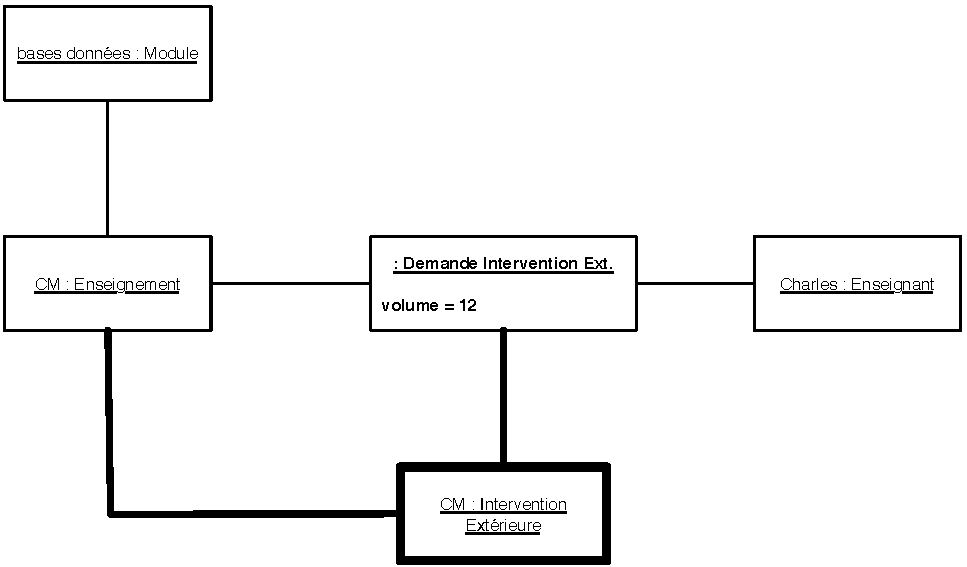
\includegraphics[scale=.6]{OD-affecter-exterieur}
\caption{Diagramme d'objets: Affectation à partir d'une demande extérieure}
\label{fig:affectation:ext}
\end{center}
\end{figure}


\subsubsection{Exemple d'affectation à partir d'une demande spéciale}
La Figure~\ref{fig:affectation:spe} présente une affectation d'une demande spéciale de congé faite par l'enseignant Eve.
L'affectation une instance de  \code{CasSpécial} associé à l'enseignant et à la demande spéciale concernés.

 \begin{figure}[!htbp]
 \begin{center}
 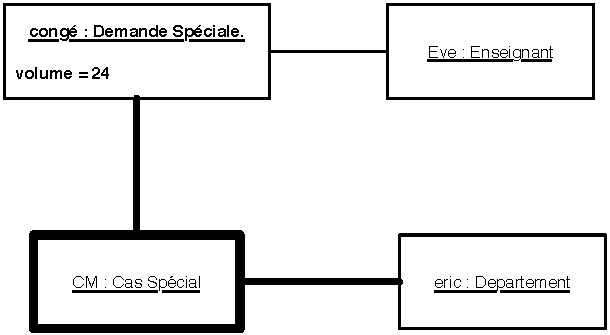
\includegraphics[scale=.6]{OD-affecter-speciale}
 \caption{Diagramme d'objets: Affectation à partir d'une demande spéciale}
 \label{fig:affectation:spe}
 \end{center}
 \end{figure}

\subsubsection{Exemple d'affectation imposée à un enseignant}
La Figure~\ref{fig:affectation:imposee} présente une affectation imposée d'un enseignement de TP à l'enseignant Alice.
L'imposition d'une intervention à un enseignant crée une instance de la classe \code{InterventionDepartement} associée à l'enseignant et à l'enseignement concernés. Les interventions (dans le département) imposées ne sont pas liées à un vœu.

\begin{figure}[!htbp]
\begin{center}
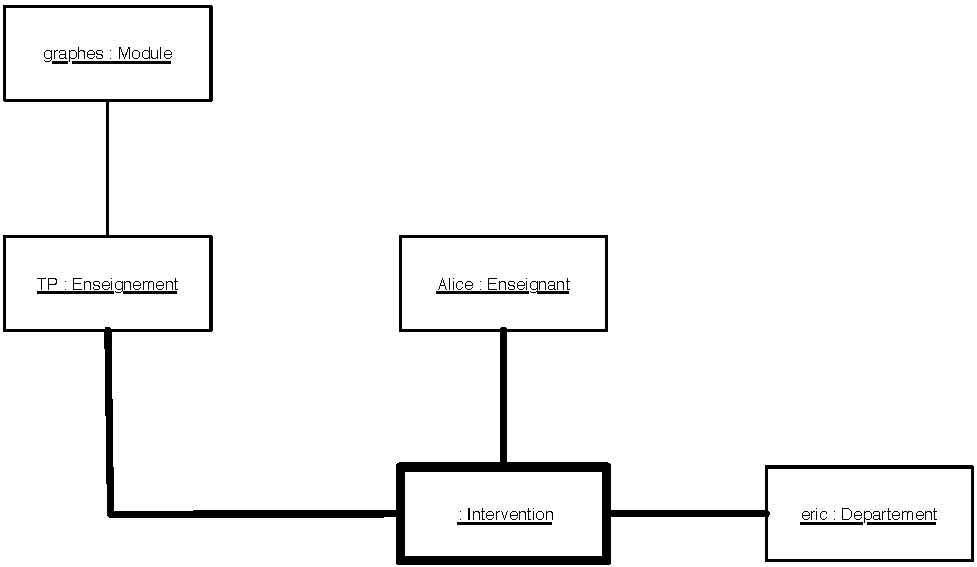
\includegraphics[scale=.6]{OD-affecter-forcee}
\caption{Diagramme d'objets: Imposition d'une intervention à un enseignant}
\label{fig:affectation:imposee}
\end{center}
\end{figure}


\begin{comment}
	

 \subsubsection{Instantané: imposition d'une intervention à un enseignant par le chef de département}
 \begin{figure}[!htbp]
 \begin{center}
 \includegraphics[width=15cm]{fig/scenario3.jpg}
 \caption{Scénario : imposition d'une intervention à un enseignant par le chef de département}
 \end{center}
 \end{figure}

 Dans ce scénario, le chef de département impose une intervention concernant un enseignement de son département. L'affectation est donc imposée à l'enseignant.  

 \subsubsection{Instantané: imposer une affectation de type ``cas spécial'' (ex : arrêt maladie)}
 \indent Cas d'utilisation : \textbf{Réaliser une affectation} - Acteur : \textbf{Chef de département}

 \begin{figure}[!htbp]
 \begin{center}
 \includegraphics[width=14cm]{fig/10-ImpositionCasSpecial.jpg}
 \caption{Imposer une affectation de type ``cas spécial'' (ex : arrêt maladie)}
 \end{center}
 \end{figure}

 \indent L'imposition d'une affectation de type ``cas spécial'' à un enseignant crée une instance de la classe \textbf{CasSpécial} associée à l'enseignant concerné. Ce ``cas spécial'' n'est pas lié à une demande spéciale (puisqu'elle a été imposée).

 \begin{ocl}
 context Departement::imposeCasSpecial(ens : Enseignant, c : CasSpecial)
 post : ens.est_affecte_pour -> include(c)
 \end{ocl}
 \emph{Le CasSpecial c, appartient à la liste des affectations de l'enseignant ens. C'est le chef de département qui impose ce CasSpecial.}


%Afin d'avoir une vue plus globale de l'application, nous avons rédigé quelques scénarii faisant intervenir différents acteurs et différents cas d'utilisation. Ces scénarii sont exprimés sous la forme de diagrammes de séquence.

 \subsubsection{Conflit entre deux enseignants - résolution par le chef de département}
 \begin{figure}[!htbp]
 \begin{center}
 \includegraphics[width=15cm]{fig/scenario1.jpg}
 \caption{Scénario : conflit entre deux enseignants - résolution par le chef de département}
 \end{center}
 \end{figure}

Dans ce scénario, le conflit est réglé par le chef de département qui affecte l'enseignement à un seul des deux enseignants (la demande de l'autre enseignant est alors considérée comme étant refusée).

 \subsubsection{Conflit entre deux enseignants - résolution par un des enseignants}
 \begin{figure}[!htbp]
 \begin{center}
 \includegraphics[width=15cm]{fig/scenario2.jpg}
 \caption{Scénario : conflit entre deux enseignants - résolution par un des enseignants}
 \end{center}
 \end{figure}

 Dans ce scénario, le conflit est réglé par un des deux enseignants qui annule son vœu concernant l'enseignement à l'origine du conflit.  

\end{comment}

\subsection{UC---Valider des souhaits et publication des possibles conflits}

\begin{usecase}{Valider des souhaits et publication des possibles conflits}
\label{usecase:publier}
\begin{information}
	
\item[{Goal in the context:}]
 Le chef de département, par cette action, permet aux autres acteurs du système (en l'occurence les enseignants) de visualiser les informations concernant l'état actuel des souhaits de l'ensemble des enseignants. 
L'exécution de ce cas d'utilisation peut faire apparaître de nouveaux conflits pour les enseignants.

\item[Scope:] Département

 \item[{Level:}] Résumé

 \item[Precondition:] aucune

 \item[{Success End Condition:}]
Les enseignants ont accès aux informations concernant l'état actuel des souhaits publiés. 
Des conflits peuvent apparaître localement pour chaque enseignant.

 \item[{Failed End Condition:}]
 Echec de la publication : les enseignants n'ont toujours pas accès aux informations que le chef de département a tenté de publier.

\item[Primary actor:] Chef de département.

 \item[{Trigger:}]
 Demande de publication des interventions, des souhaits et des conflits possibles faite par le chef de département.
\end{information}

\begin{scenario}
\item Le chef de département visualise l'ensemble des souhaits non publiés.
% \item L'application renvoie l'ensemble des information voulues.
 \item Le chef de département sélectionne un ensemble de souhait et les valide.
 \item Le chef de département rend publics les souhaits validés.
 \item Le chef de département publie les nouveaux conflits qui sont apparus après la validation.
\end{scenario}

\end{usecase}

 \subsection{UC---Analyser des demandes}

\begin{usecase}{Analyser des demandes}\label{usecase:analyse}

\begin{information}
	

\item[Goal in the context:] Le chef de département effectue une analyse statistique permettant de déterminer la répartition des volumes horaires par enseignants ou la répartition des souhaits et affectations entre enseignants pour une année donnée. 

\item[Scope:] Département

\item[{Level:}] Résumé

\item[{Precondition:}]
 /

 \item[Success End Condition:]
/
% L'utilisateur visualise le résultat de l'étude statistique.

 \item[Failed End Condition:]
 /

 \item[Primary actor:]
 Chef de département.

 \item[Trigger:]
 Demande de réalisation d'un analyse statistique faite par le chef de département.\\
\end{information}

\begin{scenario}
	\item Le chef de département visualise les affectations (interventions) et les souhaits par rapport à une année donnée, selon un critère donné: par module, par enseignant, ou par le nombre d'heures effectives ou souhaitées.
	%\item Le chef département sélectionne les données qu'il désire ``analyser''. (cas d'utilisation n°3)
	\item Le chef de département analyse et corrige les affectations d'enseignement.
\end{scenario}

\end{usecase}

\subsection{UC---Émettre un souhait}

\begin{usecase}{\'Emettre un souhait}\label{usecase:souhait}
\begin{information}

\item [{Goal in the context:}]
 L'enseignant émet un souhait. Le souhait correspond à vœu sur un ensemble d'enseignements (avec une préférence) du département, une demande d'intervention extérieure au département ou une demande spéciale (arrêt maladie, remplacement,\dots)

\item[Scope:] Département

\item [{Level:}] Summary (Résumé)

\item[{Precondition:}]
 En cas de vœux sur des enseignements, ces derniers doivent exister et être non affectés à un autre enseignant.

\item[{Success End Condition:}]
 Le souhait de l'enseignant a été pris en compte mais n'est pas encore publié c'est-à-dire que seul l'enseignant peut le voir (i.e. cette modification est locale). 
Le volume horaire total (le volume horaire effectif plus la somme des volumes horaires des souhaits pas encore validés) de l'enseignant est modifié (recalculé) par rapport au volume horaire précisé dans le souhait.

\item[{Failed End Condition:}] L'enseignent n'arrive pas à émettre son souhait.
\item[{Primary actor:}] Enseignant.
\item[{Trigger:}] Demande d'émission d'un souhait faite par l'enseignant.
\end{information}

 %\noindent\textbf{MAIN SUCCESS SCENARIO}
 \begin{scenario}
	 \item L'enseignant recopie son souhait de l'année précédente.
	 \item L'enseignant visualise l'ensemble des enseignements disponibles (i.e. non affectés) dans son département.
	 \item L'enseignant fait son choix en sélectionnant un ensemble d'enseignements et indique son niveau de préférence pour ces enseignements (voulus ou seulement souhaités).
 \end{scenario}


\begin{extension}
 \item [3a.] Le vœu génère un conflit (avec d'autres souhaits déjà rendus publics) : le système le notifie à l'enseignant.
 \item [3b.] Le souhait génère un surplus d'heures pour l'enseignant (par rapport à son contrat de services) : le système le notifie à l'enseignant.
\end{extension}


\begin{variation}
	\item [1.] L'enseignant ne possède pas de historique de souhaits. Il commence avec un ensemble vide de souhaits.
	\item [3.] L'enseignant fait une demande concernant une intervention extérieure au département, précise le volume horaires et l'organisme concerné.
	\item [3.] L'enseignant décide de faire une demande spéciale souhaité en précisant le type (un congé, un remplacement, \dots) et le volume horaire.
\end{variation}
\end{usecase}

\subsubsection{Spécification OCL}
\begin{ocl}
context UC::EmettreVoeu(ens:Enseignant, m:Module, e:Enseignement, h: Integer, p:Integer)
post: 
ens.voeux->exists(v:Voeu| v.enseignement = e and v.volume = h and v.priorite = p)

-- Un nouveau voeu est ajouté à la liste des voeux de l`enseignant
\end{ocl}

\begin{ocl}
context UC::EmettreDemandeExterieure(ens:Enseigant, org:String, vol:Integer)
post: 
	ens.demandes->select(each | each.oclIsTypeOf(DemandeInterventionExterieure))->
		exists(d | d.oclIsNew() and d.volume = vol and d.organisation = org)
		
-- Une nouvelle demande d`intervention à l`extérieur est ajoutée à la liste de demandes de l`enseignant.
\end{ocl}

\begin{ocl}
context UC::EmettreDemandeSpeciale(ens:Enseignant, t:String, vol:Integer)
post:
	ens.demandes->select(each | each.oclIsTypeOf(DemandeSpeciale))->
		exists( d | d.oclIsNew() and d.volume = vol and d.type = t)

-- Une nouvelle demande spéciale est ajouté à la liste de demandes de l`enseignant.
\end{ocl}


\subsubsection{Exemple d'émission d'un souhait}
Dans cet exemple, l'enseignant Alice émet le souhait de réalise deux enseignements:
\begin{enumerate}
	\item Enseignement de 16h de CM du module Génie Logiciel;
	\item Enseignement de 16h de TD du module Réseaux.
\end{enumerate}
Le diagramme d'objets présenté dans la Figure~\ref{fig:souhait-alice} illustre ce souhait.
Après l'émission du souhait, une instance de la classe \code{Voeu} est créée pour chaque vœu, ainsi que deux liens, avec l'enseignant et l'enseignement concernés. 

 \begin{figure}[!htbp]
 \begin{center}
 \includegraphics[scale=.6]{"OD-alice-demande-gl"}
 \caption{Diagramme d'objets: Alice émet son souhait de service}
 \end{center}
 \label{fig:souhait-alice}
 \end{figure}


 \subsubsection{Exemple d'émission d'une demande extérieure}
Dans cet exemple, l'enseignant Bob fait une demande d'intervention de 12h à l'Institut Mines-Télécom Atlantique.
Le diagramme d'objets présenté dans la Figure~\ref{fig:demande:exterieure} illustre cette demande.
L'émission d'une demande extérieure crée une nouvelle demande extérieure associée à l'enseignant.
 
 \begin{figure}[!htbp]
 \begin{center}
 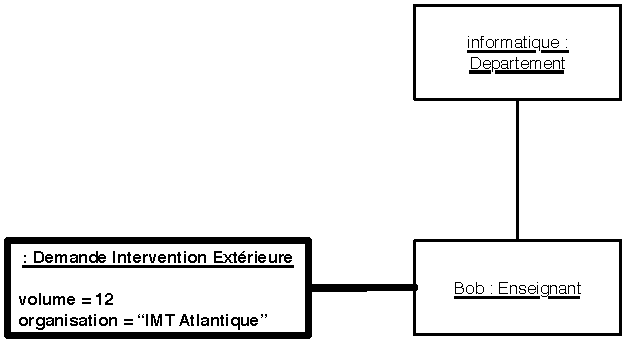
\includegraphics[scale=.6]{OD-emettre-demande-exterieure}
 \caption{\'Emission d'une demande d'intervention extérieure}
 \label{fig:demande:exterieure}
 \end{center}
 \end{figure}

 \subsubsection{Exemple d'émission d'une demande spéciale}
Dans cet exemple, l'enseignant Charles fait une demande de congés paternité, qui équivaut à 12h de décharge de service.
L'émission d'une demande spéciale crée la demande spéciale associée à l'enseignant.
\begin{figure}[!htbp]
\begin{center}
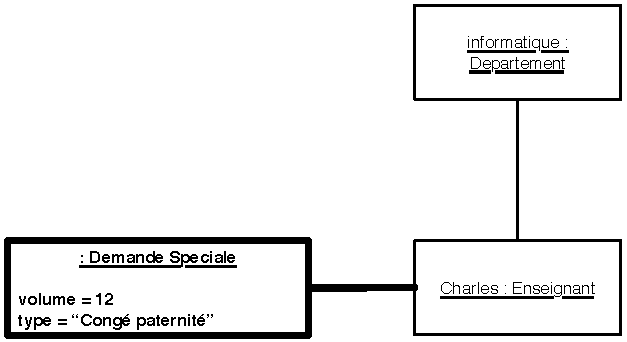
\includegraphics[scale=.6]{OD-emettre-demande-speciale}
\caption{\'Emission d'une demande spéciale}
\end{center}
\end{figure}




\subsection{UC---Publier des souhaits}
\begin{usecase}{Publier des souhaits}
\label{usecase:publier}
\begin{information}
	\item[Goal in the context:] L'enseignant transmet ses souhaits (préalablement sélectionnés) au chef de département qui sera lui même apte, dans un deuxième temps, à les rendre visibles à l'ensemble des enseignants.
Un souhait concerne un vœux fait sur des enseignements disponibles (i.e. non affectés), une intervention extérieure au département ou bien encore une demande caractérisée comme étant spéciale (congé, remplacement, \dots). 
	\item[Scope:] Département
	\item[Level:] Résumé
	\item[Precondition:] Le ou les vœux concernés ont été préalablement réalisés et validés localement par l'enseignant.
	\item[Success End Condition:] Le chef de département est capable de visualiser le/les souhaits publiés par l'enseignant.
	\item[Failed End Condition:] Le département ne reçoit pas les souhaits de l'enseignant.
	\item[Primary actor:] Enseignant.
	\item[Trigger:] Demande de publication de souhaits faite par l'enseignant.
\end{information}
\end{usecase}


\begin{scenario}
	\item L'enseignant choisit de visualiser l'ensemble des souhaits qu'il a réalisé localement mais qu'il n'a pas encore publié.
%	\item Le système lui renvoie l'ensemble de ces souhaits classés selon leur type (i.e. vœu, intervention extérieure et demande spéciale)
	\item L'utilisateur choisit, parmi ces souhaits, ceux qu'il désire publier et les transmet au chef de département.
	\item Le chef du département reçoit les vœux de l'enseignant.
\end{scenario}

 \begin{extension}
	 \item [2a.] Le système lui signifie qu'il n'existe pas de souhaits qui sont en attente d'être publiés.
	 \item [3a.] L'enseignant décide de ne publier aucun de ces souhaits et annule sa demande de publication.
	 \item [4a]. Le système signifie à l'utilisateur que l'un de ces souhaits (en l'occurence un vœu) concerne un ou plusieurs enseignements qui ont été affectés ou supprimés et lui demande de modifier son vœu.\\
 \end{extension}


 \subsection{UC---Consulter des enseignements}

\begin{usecase}{Consulter des enseignements}
\label{usecase:consulter}
\begin{information}
	\item[Goal in the context:]  L'enseignant doit être capable de visualiser les enseignements afin de consulter ou de modifier ses souhaits.
 Ainsi, des critères de tri sont mis à sa disposition pour personnaliser sa vue des enseignements dans le système "\projet": par module, par enseignement d'un module, par enseignant, ou par nombre d'heures.\\
 De plus, il doit choisir les critères de sélection des enseignements qu'il souhaite visualiser:
Les enseignements concernés par des vœux publiés ou non; les enseignements concernés par des vœux déjà validés (affectations);
ou les enseignements affectés et ceux non affectés.\\
 L'enseignant peut choisir de visualiser les enseignements des années précédentes mais il ne pourra effectuer aucune modification sur ces années. Par défaut, la visualisation se fera sur l'année en cours.
 L'utilisateur choisit l'ensemble des critères de tri et de sélection sur les enseignements qu'il souhaite. Il peut donc entièrement paramétrer sa vue des enseignements.
	\item[Scope:] Département
	\item[Level:] Résumé
	\item[Precondition:]/
	\item[Success End Condition:]/
	\item[Failed End Condition:]/
	\item[Primary actor:] Enseignant.
	\item[Trigger:] Demande de consultation des enseignements selon différents critères faite par l'enseignant.
\end{information}

\begin{scenario}
	\item L'enseignant décide de visualiser l'ensemble des enseignements selon ses critères.
	\item Le système renvoie l'ensemble des enseignements correspondants aux critères demandés.
\end{scenario}

 \begin{extension}
 \item [2a.] Le système ne renvoie rien puisqu'aucun enseignement ne correspond aux critères demandés.
 \end{extension}
\end{usecase}


\begin{comment}
 %*********
 \subsection{Instantanés et contraintes OCL sur les cas d'utilisation}
 \indent Nous allons vous présenter, dans cette sous-partie, un ensemble représentatif d'instantanés des cas d'utilisation. Nous allons donc partir d'un système vide (seul le département est représenté avec un module et deux enseignements) pour ensuite illustrer l'évolution de notre système au cours de son utilisation.\\
 \indent Voici le diagramme d'instances qui va nous servir de point de départ pour nos instantanés (nous considérons comme triviale la création des modules et des enseignements associés à un département) :

 \begin{figure}[!htbp]
 \begin{center}
 \includegraphics[width=4cm]{fig/base.jpg}
 \caption{Instantané de départ}
 \end{center}
 \end{figure}

 \subsubsection{Assigner un enseignant à un département}
 \indent Cas d'utilisation : non mentionné car basique - Acteur : \textbf{Chef de département}.

 \begin{figure}[!htbp]
 \begin{center}
 \includegraphics[width=12cm]{fig/1-assignEnseignant.jpg}
 \caption{Assignation d'un enseignant}
 \end{center}
 \end{figure}

 \indent L'assignation d'un nouvel enseignant au département provoque l'ajout d'une instance de la classe \textbf{Enseignant} ainsi que du contrat de service qui lui est associé (instance de la classe \textbf{ContratDeService}).

 \begin{verbatim}
 context Departement::assignerEnseignant(e : Enseignant)
 post : self.enseignant.include(e)
        and not e.contratdeservice.isUndefined()
 \end{verbatim}
 \emph{L'enseignant appartient au département et possède un contrat de service unique. L'assignation provient du chef de département.}







 \subsubsection{Assigner un responsable à un module}
 \indent Cas d'utilisation : \textbf{Assigner un responsable} - Acteur : \textbf{Chef de département}.

 \begin{figure}[!htbp]
 \begin{center}
 \includegraphics[width=12cm]{fig/4-ResponsableModule.jpg}
 \caption{Assignation d'un responsable à un module}
 \end{center}
 \end{figure}

 \indent L'assignation d'un responsable de module associe un enseignant au module dont il devient le responsable.

 \begin{verbatim}
 context Departement::assignerResponsable(m : Module, ens : Enseignant)
 post : m.est_responsable_de = ens
 \end{verbatim}
 \emph{L'enseignant ens devient responsable du module m. Cette assignation est réalisée par le chef de département}
\end{comment}

 \section{Diagramme de classes métiers}
Afin d'achever cette phase de spécification des besoins, nous fournissons une modélisation statique et synthétique du domaine de notre application. La figure~\ref{cls-metier} représente ce domaine "Gestion des services": 

 \begin{figure}[!htb]
 \centering
 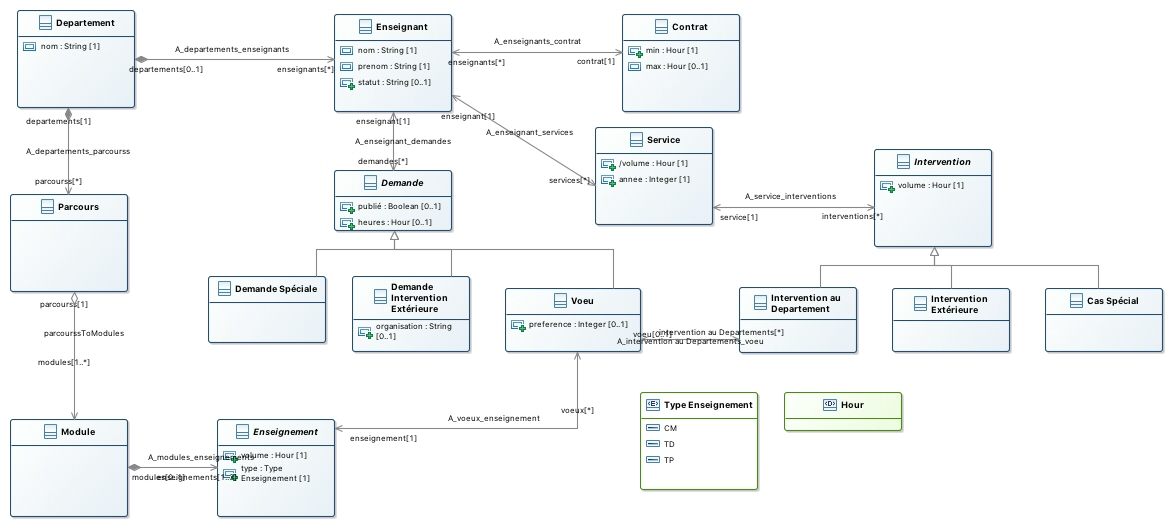
\includegraphics[width=\linewidth] {CD-Gestion Services.jpg}
 \caption{Diagramme de classes métiers du domaine ``Gestion des services''}
 \label{cls-metier}
 \end{figure}

Le domaine "Gestion des services" est composé d'un ensemble de départements identifiés par leur nom (ex: département ``Informatique'', département ``Mathématiques'', \dots). 
Chacun de ces départements est constitué de parcours et possède un certain nombre d'enseignants qui lui sont rattachés.
Un parcours a un nom (ex: "Licence informatique", "Master Alma", etc.).

 Un module est défini par un nom, une année d'étude (ex: 2$^{\textrm{\footnotesize{e}}}$ année) et un semestre (1$^{\textrm{\footnotesize{e}}}$ ou 2$^{\textrm{\footnotesize{e}}}$). Il se décompose en plusieurs enseignements avec pour chacun un volume horaire et un coefficient: il peut s'agir de cours magistraux (CM), de travaux dirigés (TD) ou de travaux pratiques (TP). 
Chaque module a pour responsable un enseignant qui se doit, en principe, d'assurer un certain nombre d'enseignements dans ce module (le plus souvent les cours magistraux).

 Les enseignants sont caractérisés par leur nom et leur statut et doivent chacun remplir un contrat de service par année, c'est-à-dire effectuer un certain nombre d'heures minimum d'enseignement par année (calculé à partir des coefficients des enseignements). Il est important de noter que le contrat de service est uniquement fonction du statut de l'enseignant et est indépendant du département auquel il est rattaché.

 Chaque enseignant peut émettre un certain nombre de souhaits afin d'indiquer la manière dont il désire remplir son contrat de service. Ces souhaits peuvent être des vœux (indications du ou des enseignements que l'enseignant souhaite dispenser ainsi que ses préférences les concernant), des demandes d'intervention extérieure (dans une entreprise, une autre école...) ou des demandes spéciales (congés, arrêts maladie, encadrements de stages ou de TER\dots).

 Il est ensuite du ressort du chef du département concerné de décider de valider ou non ces souhaits, i.e. d'affecter ou non à l'enseignant concerné les interventions correspondantes aux souhaits émis. Toutefois, pour régler certains conflits, le chef d'un département se réserve le droit d'imposer une affectation à un enseignant sans que cet enseignant en ait auparavant formulé le souhait.

 % Pour terminer, notons que l'attribut nommé "année", présent dans la classe "Département", permet d'assurer la persistance des données concernant les modules, les enseignants, les souhaits et les interventions des différents enseignants au fil des années. Ainsi, il sera possible de construire un historique des souhaits et des interventions dans notre système. Cela pourra s'avérer très utile afin de permettre au chef de département de tenir compte des demandes des années passées pour le guider dans ses choix d'affectation concernant l'année en cours. Nous ne nous étendons pas sur le sujet de la persistance puisque ce n'est pas l'objectif de la phase de spécification des besoins.



%!TEX root = /Users/sunye/Development/Workspaces/teaching/Gestion services/src/doc/latex/sujet-projet.tex

\chapter{Dictionnaire de données}

Dans une première partie, nous fournissons le dictionnaire des données que nous avons construit suite `a notre analyse du cahier des charges. Il s’agit d’un listing de l’ensemble des termes relatifs au domaine étudié (`a savoir le domaine “Gestion des services”) ainsi que leur définition précise.


\begin{longtable}{p{3cm}p{8cm}p{2cm}p{2cm}}

\toprule
\textbf{Notion} & \textbf{Définition} &\textbf{Traduit en} & \textbf{Nom informatique} \\
\midrule

Affectation & Action de déterminer une \textbf{intervention}, i.e. d'associer un \textbf{enseignant} à un \textbf{enseignement} donné. C'est le \textbf{chef de département} qui est chargé de déterminer les différentes affectations en fonction, le plus souvent, des \textbf{v\oe ux} réalisés par les divers \textbf{enseignants}. & &\\

Chef de département & Acteur du système. Il est le responsable d'un \textbf{département} : il gère les \textbf{modules} (ainsi que les \textbf{enseignements} associés), les \textbf{enseignants} et leurs \textbf{interventions} pour son \textbf{département}. & Acteur & ChefDepartement \\

Conflit & Fait que deux \textbf{v\oe ux} soit incompatibles (i.e. que deux \textbf{enseignants} aient émis les mêmes choix concernant un ou des \textbf{enseignements}). C'est au \textbf{chef de département} de régler les conflits en réalisant les affectations. & &\\

Contrat de service & Nombre d'heures minimum (et parfois nombre d'heures maximum) d'\textbf{enseignements} à effectuer pour un \textbf{enseignant} donné. Il est indépendant des \textbf{départements} dans lesquels l'\textbf{enseignant} intervient : il est unique et seulement déterminé par le statut de l'\textbf{enseignant}. & Classe & ContratDeService \\

Département & Entité administrative (d'une université) identifiée par un nom. Il comprend un ensemble de \textbf{modules} et d'\textbf{enseignants} qui lui sont rattachés. Chaque département a pour responsable un \textbf{chef de département}. Plusieurs \textbf{enseignants} peuvent donner des \textbf{enseignements} pour le compte de chaque \textbf{département}. & Classe & Departement  \\

Enseignant & Personne "physique" travaillant pour le compte d'un \textbf{département} et identifiée par son nom, son prénom et son statut. Un enseignant peut "intervenir" dans différents \textbf{départements} pour dispenser un certain nombre d'\textbf{enseignements}. C'est un également un acteur du sytème puisqu'il peut effectuer des \textbf{v\oe ux} concernant les \textbf{enseignements} qu'il désire donner. & Classe et Acteur & Enseignant \\

Enseignement & Entité administrative représentant un cours dans un \textbf{module} donné. Il existe trois types d'enseignement avec, pour chacun, un coefficient différent en terme de volume horaire:
\begin{itemize}
\item CM : cours magistral se déroulant le plus souvent dans un amphithéâtre, un CM vaut 3/2 d'un TD ;
\item TD : travaux dirigés se déroulant dans une salle de cours classique ;
\item TP : travaux pratiques se déroulant dans des salles particulières dédiées à cet effet (salles machines, laboratoires...), un TP vaut 2/3 d'un TD (ou 1 TD, cela dépend du statut de l'\textbf{enseignant} concerné).
\end{itemize} & Classe & Enseignement, CM, TD, TP \\

Intervention & Fait qu'un \textbf{enseignant} intervienne dans un \textbf{département} donné. Elle a pour origine, la plupart du temps, un \textbf{souhait} formulé par un \textbf{enseignant}. Cette intervention peut être de différentes natures:
\begin{itemize}
\item il peut s'agir d'une intervention dans le département, c'est-à-dire qu'un \textbf{enseignement} soit affecté à un \textbf{enseignant} pour un volume horaire donné;
\item il peut s'agir d'une intervention extérieure (dans une entreprise, une autre école...), d'un volume horaire donné ;
\item il peut s'agir d'un cas spécial (congés, maladies, encadrement d'un stage ou d'un TER...), toujours d'un volume horaire donné.
\end{itemize} & Classe & Intervention, InterventionDépartement, InterventionExtérieure, CasSpécial \\

Jouer & Terme employé dans la description du domaine. Action, faite par un \textbf{enseignant}, de formuler un certain nombre de \textbf{souhaits} qu'il pourra décider, par la suite, de publier (de soumettre au \textbf{chef de département} et aux autres \textbf{enseignants}) ou pas. & &\\ 

Module & Entité administrative (d'un \textbf{département}) regroupant un ensemble d'\textbf{enseignements} concernant un sujet donné. Chaque module est identifié par un nom (intitulé du module) et caractérisé par une année d'étude, un nom de parcours et un semestre. & Classe & Module \\

Publication & Action de rendre public (i.e. accessible à tous les utilisateurs du système, qu'ils soient \textbf{enseignant} ou \textbf{chef de département}) un ou des \textbf{souhaits} formulés par un ou des \textbf{enseignants}. & Attribut & "publié" dans la classe Souhait \\

Souhait & Fait qu'un \textbf{enseignant} effectue une demande d'un certain type concernant les interventions qu'il souhaite réaliser pour remplir son \textbf{contrat de service}. Ce souhait peut être :
\begin{itemize}
\item un \textbf{v\oe u};
\item une demande d'intervention extérieure (dans une autre école, une entreprise...) d'un volume horaire donné;
\item une demande spéciale (congé, arrêt maladie, encadrement d'un stage ou d'un TER...) d'un volume horaire donné.
\end{itemize}

Un souhait peut être à l'origine d'une \textbf{intervention} affectée (déterminée) par le \textbf{chef de département} (ou plusieurs dans le cas d'un \textbf{v\oe u}).
& Classe & Souhait, Voeu, DemandeInterventionExtérieure, DemandeSpéciale \\

V\oe u & Choix fait par un \textbf{enseignant}, pour un \textbf{département} donné, indiquant quels \textbf{enseignements} il désire dispenser ainsi que ses préférences concernant ces \textbf{enseignements}. Les préférences pour un \textbf{enseignement} sont déterminées de la manière suivante:
\begin{itemize}
\item 1 : si cet \textbf{enseignement} est réellement souhaité par l'\textbf{enseignant};
\item 0 : si cet \textbf{enseignement} est toléré par l'\textbf{enseignant}.
\end{itemize} 
Un v\oe u pourra, après validation par le \textbf{chef de département}, faire l'objet d'une ou plusieurs \textbf{interventions}. & Classe & V\oe u \\
\bottomrule
\end{longtable}

%!TEX root = ./sujet-projet.tex

\chapter{Architecture}

\section{Introduction}
	Dans ce chapitre, vous devez fournir une description générale de l'architecture de votre système et décrire comment vous répondez aux exigences non-fonctionnelles énoncés précédemment dans la Section~\ref{section:non-fonctionnelles}.


\section{Vue physique}

Utilisez un diagramme de déploiement UML pour décrire l'architecture physique de l'application: les nœuds logiques, les protocoles de communication, le déploiement des artefacts logiciels (bibliothèques, autres logiciels, etc.).
N'oubliez pas de décrire votre diagramme.

Si l'architecture physique répond à une ou des exigences logicielles, n'oubliez pas de le mentionner.

\begin{figure}[!htbp]
\begin{center}

\caption{Diagramme de déploiement du système ``\projet{}''}

\end{center}
\end{figure} 

Utilisez également le diagramme de déploiement, mais au niveau instance, pour fournir des exemples de déploiement du système.

\begin{figure}[!htbp]
\begin{center}

\caption{Diagramme d'instances modélisant un déploiement possible du système ``\projet{}''}
\end{center}
\end{figure} 


\section{Vue du développement}
Utilisez le diagramme de paquetages UML pour décrire l'organisation du code source de votre application.
N'oubliez pas de le commenter.

Si l'architecture logique répond à une ou des exigences logicielles, n'oubliez pas de le mentionner.

\section{Vue logique}

Présentez ici les composant principaux du système.

\begin{figure}[!htbp]
\begin{center}
\caption{Diagramme d'instances modélisant un déploiement possible du système ``\projet{}''}
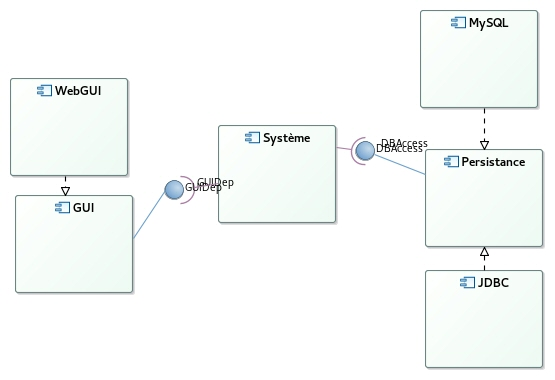
\includegraphics[scale=.7]{Vue_composants.jpg}
\end{center}
\end{figure} 

\section{Vue des processus}
Présentez ici les différents processus d'exécution dans votre système.

\section{Vue de la fiabilité}

Énumérez ici les choix architecturaux faits pour assurer la fiabilité du système.


\section{Réponses aux exigences non-fonctionnelles}
Expliquez, dans cette section, la réponse de votre solution aux exigences non-fonctionnelles. 
Les sous-sections présentées ici ne constituent pas une liste exhaustive. 

\subsection{Gestion de la concurrence}

\subsection{Gestion de la persistance}

\subsection{Gestion de la sécurité}


\section{Architecture technique : traduction de UML en code source}
Expliquez, dans cette partie, l'ensemble de règles que vous utiliserez par la suite pour traduire nos diagrammes \textsc{UML} (découlant de notre analyse et de notre conception) en code source (classes d'implémentation).\\ 

\subsection{Règles de traduction des types de base}

\subsection{Règles de traduction des classes}

\subsection{Règles de traduction des associations, agrégations composites et agrégations partagées}

\subsection{Règles de traduction des composants}

\subsection{Autres règles}



\section{Patrons architecturaux utilisés}

Fournissez, dans cette dernière partie, une liste exhaustive des patrons de conception que vous allez utiliser pour mettre en œuvre notre application. 
Pour chacun de ces patrons, donnez une courte description ainsi que les raisons pour lesquelles vous avez choisi de les mettre en \oe uvre.\\


\subsection{Patron A}

\subsection{Patron B}

\subsection{Patron C}

\subsection{Patron D}

\subsection{Patron D}

\subsection{Patron E}


\section{Choix techniques - Distribution des processus}

\indent Nous allons ici expliciter les différents choix techniques que nous avons choisit et les réponses technologiques aux différentes contraintes que notre système implique. Nous allons donc vous présenter l'environnement général de développement puis énoncer les 4 contraintes que nous avons déterminées de notre logiciel.

%
%  Choix de l'environnement  
%



\section{Conclusion}


%!TEX root = ./sujet-projet.tex

%
% Spécification des composants
%
\chapter{Spécification des composants}\label{chapter:composants}

\section{Introduction}

	\subsection{Objectif}
Préciser les objectifs de ce chapitre. 

	\subsection{Organisation du chapitre}
Cette section décrit le contenu du reste du chapitre  et explique comment le document est organisé.
\section{Description des composants}

Établir les frontières du système.

Division du système en composants.

Décrire le comportement souhaité des composants.

\subsection{Le composant A}

\begin{figure}[htbp]
	\centering
%		\includegraphics[scale=1]{file}
	\caption{Le composant A et ses interfaces}
	\label{fig:label}
\end{figure}

\section{Interactions}

Décrivez, à haut-niveau, la collaboration entre les composants majeurs, pendant la réalisation des cas d'utilisation. 
Utilisez des interactions, c'est à dire, des diagrammes de séquence et des diagrammes de communication, pour décrire les cas nominaux et extra-nominaux des cas d'utilisation.


\emph{Ne vous limitez pas à une seule interaction par cas d'utilisation}

\subsection{Cas d'utilisation UC1}

\begin{figure}[htbp]
	\centering
		% \includegraphics[scale=1]{file}
	\caption{Interaction \--- Création d'une tâche}
	\label{fig:label}
\end{figure}

\begin{figure}[htbp]
	\centering
		% \includegraphics[scale=1]{file}
	\caption{Interaction \--- Création d'une tâche répétitive}
	\label{fig:label}
\end{figure}

\section{Spécification des interfaces}

	\subsection{Interface A}
	
	Présentation de l'interface en UML (ou HUTN). Description du comportement de chaque opération. Spécification éventuelle des pré-conditions en OCL.
	
\begin{itemize}
	\item \code{getTasksForDate(Date) : Task[*]} \\
	Retrouve un ensemble de tâches pour une date donnée.
\begin{ocl}
getTasksForDate(Date) : Task[*]
pre: 
-- Le package \emph{listings} n'est pas compatible avec UTF8.
-- Donc, n'utilisez pas d'accent.
\end{ocl}
	
	\item \code{removeAllTalks()} \\
	Efface toutes les tâches, éteint le serveur et débranche son câble de la prise électrique.
	
	\item \code{getTaskForNamde(String, Number) : Task} \\
	Retrouve une tâche à partir de son nom et son numéro de téléphone.
\end{itemize}	
	\subsection{Interface B}
	
	\subsection{Interface C}

\section{Spécification des types utilisés}

Spécifiez ici les types utilisés par les interfaces (seulement ceux qui ne font pas partie des types de base UML).

\subsection{Task}

	La classe \code{Task} représente une Tâche. Elle possède les attributs suivants:
	\begin{description}
		\item[name]: le nom de la tâche. 
		\item[isActive]: détermine si la tâche est activée ou non.  
	\end{description}

\begin{figure}[htbp]
	\centering
%		\includegraphics[scale=1]{task}
	\caption{La classe Task}
	\label{fig:taks}
\end{figure}

\section{Conclusion}

%!TEX root = ./sujet-projet.tex

\chapter{Conception détaillée}

\section{Introduction}

\section{Répertoire des décisions de conception}

Cette section doit contenir un répertoire regroupant l'ensemble de nos décisions de conception concernant votre système.

Si vous utilisez des patrons de conception, ou \emph{design patterns}, décrivez leur utilisation dans les sections suivantes.

\subsection{Patron A}
Description de l'utilisation.

\subsection{Patron B}
Description de l'utilisation.

\subsection{Patron C}
Description de l'utilisation.



%*******************************************************************
%************** Spécification détaillée des composants *************
%*******************************************************************


\section{Spécification détaillée des composants}
Cette section doit contenir une description détaillée de chacun des composants du système, dont l'interface a été présentée dans le Chapitre~\ref{chapter:composants}.

Décrivez, pour chaque composant, sa structure sous la forme d'un diagramme statique (en l'occurence un diagramme de classes avec paquetages) et son comportement interne sous la forme de diagrammes dynamiques. 

Comme UML propose plusieurs types de diagrammes statiques, pensez à bien choisir le diagramme qui permet de mieux spécifier ce que vous souhaitez décrire:
\begin{enumerate}
	\item Les diagrammes d'activités sont utiles à description d'algorithmes non-triviaux, comme la résolution de conflits, par exemple.
	\item Les diagrammes état-transition sont utilises à décrire des comportements qui dépendent de l'état interne d'un composant ou d'une classe.
	\item Les itérations sont utiles à la description d'enchainement de messages entre objets. Ils sont très utilises pour décrire des comportement nominaux et extra-nominaux, qui peuvent se traduire en tests.
\end{enumerate}

N'oubliez pas que les deux premiers diagrammes représentent des classes et des opérations, alors que le dernier représente des objets et des messages envoyés entre ces objets. Ils ne sont pas au même niveau. 



\subsection{Composant A}

\subsubsection{Structure}


\begin{figure}[!htbp]
\begin{center}

\caption{Diagramme de classes du composant A}
\end{center}
\end{figure}
 
\subsubsection{Comportement}

\begin{figure}[!htbp]
\begin{center}
\caption{Diagramme état-transition du composant A}
\end{center}
\end{figure}

Explications détaillées.

\begin{figure}[!htbp]
\begin{center}
\caption{Diagramme d'activités de l'opération \code{a()} du composant \code{A}}
\end{center}
\end{figure}

Explications détaillées.

\begin{figure}[!htbp]
\begin{center}
\caption{Diagramme de séquences de l'opération \code{a()} du composant \code{A} (cas nominal)}
\end{center}
\end{figure}
Explications détaillées.

\begin{figure}[!htbp]
\begin{center}
\caption{Diagramme de séquences de l'opération \code{a()} du composant \code{A} (cas extra-nominal)}
\end{center}
\end{figure}

Explications détaillées.


\subsection{Composant B}
\subsection{Composant C}
\subsection{Composant D}

%*******************************************************************
%************** Spécification détaillée des classes ****************
%*******************************************************************

\section{Spécification détaillée des classes}
Décrivez, dans cette section, les classes ou les opérations dont la mise en œuvre est complexe.
Il ne s'agit pas de spécifier toutes les classes et opérations, mais seulement celles dont la traduction en code n'est pas triviale.

Utilisez le langage OCL et des diagrammes dynamiques pour les décrire.


\section{Conclusion}






\bibliographystyle{plain}
\bibliography{alma} 

\end{document}
